\begin{homeworkProblem}
	\chapter{Project Plan}
	\section{Planning Process}
	Throughout the project we embodied the principles of agile development. At any point in time during our development we had working code on the master branch and every member of the team was brought up to speed with what has been completed and worked on. All goals for the project were put on Github and as they were resolved they were cleared. We created several milestones which captured our goals for completing the parser, scanner, analyzer, codegen, and final report milestones. We also  worked closely with Professor Edwards at Columbia University to receive guidance on how best to implement this language. 
	The following milestones were created and cleared over the course of the semester:
	\begin{figure}[!ht]
		\centering
		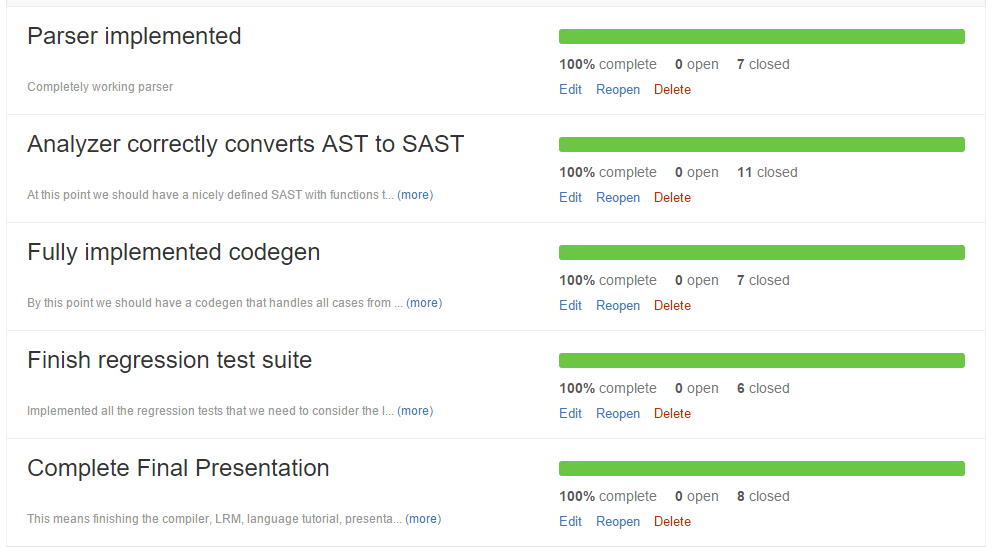
\includegraphics[width=4.5in]{Includes/milestones}
		\caption{Milestoning on Github.}
	\end{figure}
	
	\section{Specification Process}
	At the beginning of the semester we had originally intended our language to be a distributed software solution that would conveniently allow the developer to distribute tasks to various slave machines that had compiled the tasks to LLVM IR. After discussing this with professor Edwards we then decided to opt for an object oriented programming language that specifically compiled to LLVM IR. This way we as a team could learn more about making compilers and showing the power of LLVM. 
	
	Once we decided on the theme of Dice, we met to discuss the features we wanted most in our object oriented language. In our case we wanted arrays, inheritance, objects, and file IO to be some of the key highlights of our language. We then built up the scanner and parser to get a more solid idea as to what the language would look like, and by November 15th we had solidified our plans to implement the aforementioned features. 
	
	\section{Development Process}
	Implementation was very dependent on the course deadlines. We started with the scanner and parser specifically so the language reference manual was better defined. This was completed by October 26th. We then iterated on the analyzer and codegen until it was capable of producing hello world. This was completed on November 15th. The month afterwards was spent implementing inheritance and arrays until they were finally completed on December 18th. 
	
	\section{Testing Process}
	Throughout the development process we had numerous tests. The plan was to always have tests that were non-functional so a feature could then be implemented to get them working. If we encountered an error that we were unsure of how to fix, we added more error messages in our compiler until we could exactly pinpoint where the error was occurring. We also made a rule for our team to handle each and every exception that could occur as a custom error message to be printed out by the compiler. 
	
	\section{Team Responsibilities}
	Team responsibilities were divided up and evenly distributed amongst the four group members. While we could not adhere to a strict division of labor based on group member titles, every member contributed to the codebase. \\
	
	\begin{tabular}{|c|c|}
		\hline
		Team Member & Responsibility \\
		\hline
		David Watkins & Scanner, Parser, Analyzer, Codegen, Utils, LRM, Final Report, Latex, Code cleanup\\
		\hline
		Emily Chen & Inheritance in Analyzer, Expression types in Analyzer, LRM\\
		\hline
		Khaled Atef & Test Suite, Binary and unary expression evaluation in codegen\\
		\hline
		Phillip Schiffrin & Standard Library, Class map generation \\
		\hline
	\end{tabular}
	
	\section{Github Usernames}
	The following Github usernames correspond to the following group members:
	\begin{itemize}
		\item Emily Chen - six5532one, ec2805
		\item Khaled Atef - KhaledAtef
		\item David Watkins - DavidWatkins
		\item Phillip Schiffrin - nethacker11
	\end{itemize}
 
	\section{Project Log}
	To demonstrate our timeline we captured the number of git commits over time for our project. 
	
	\begin{figure}[!ht]
		\centering
		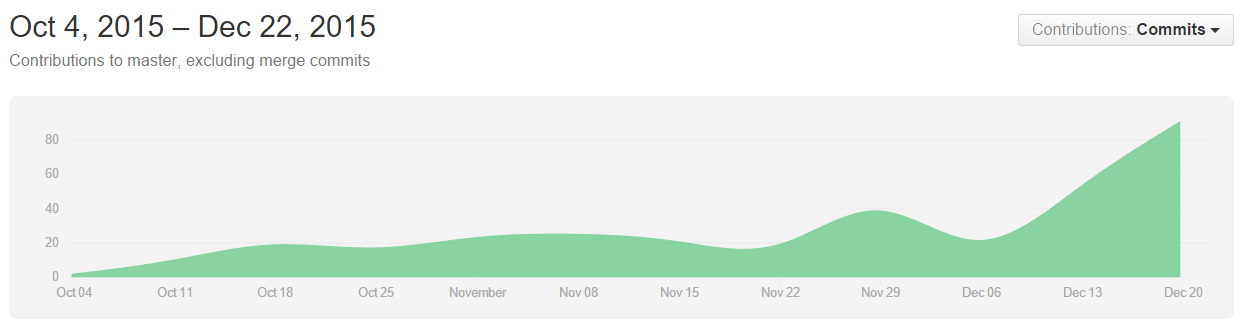
\includegraphics[width=5.5in]{Includes/timeline}
		\caption{Commit timeline on Github.}
	\end{figure}
	\pagebreak
	The timeline shows that we have been diligent at constantly working on the project since the beginning of the semester. All group members have contributed to this project. The following issues are a list of git issues that were cleared as part of our project, as well as the person who closed the issue. We did not have a rule for who closed an issue so sometimes the person who completed the issue may not have been the one to close it. 
	
	\begin{itemize}
		\item \#71 Should not be able to access variables outside of scope
		\item \#137 Awesome!
		\item \#134 Subclass assignment [by @six5532one, @DavidWatkins]
		\item \#133 string length tests
		\item \#132 fix delete test, no multiple arrays
		\item \#131 this should raise no exceptions
		\item \#130 Expected stderr: "exception Exceptions.LocalAssignTypeMismatch("B", "C")"
		\item \#129 passing in an inherited class for classes
		\item \#128 E-test-privateFieldsAccess.dice
		\item \#127 Create test for cyclical inheritance
		\item \#126 Add error message for assigning parameters
		\item \#125 test-gcd.dice Bug. You cannot assign values to parameters
		\item \#124 test-constructor1.dice is written incorrectly
		\item \#123 Maximum float is limited to 6 digits after the decimal
		\item \#122 char[][] args does not work in main
		\item \#121 Test max/min floats
		\item \#120 Test default constructor
		\item \#119 Test overloading std-lib functions
		\item \#118 Exit not working in runtime
		\item \#117 Test args
		\item \#116 assign ints to floats
		\item \#115 Integer toString generates string twice
		\item \#114 concat adds an extra character to the string
		\item \#113 Test exit
		\item \#111 Errors.log from script output isn't working properly
		\item \#110 add teststdlib .out
		\item \#109 Add Test returning objects
		\item \#108 add tests for empty blocks
		\item \#107 For inheritance of functions we should have an id to determine which function to call
		\item \#106 Includes should check with String\_lit not ID
		\item \#105 Odd invalid numbering of blocks bug
		\item \#104 Fix parameters on library functions
		\item \#103 Get Dice exec working so tests can run again.
		\item \#102 "Get the t-shirts made"
		\item \#101 Adapt codegen to changes in analyzer that add inherited fields to sprogram.classes
		\item \#100 Need to test includes
		\item \#99 add test for empty conditionals
		\item \#98 add empty for loop test
		\item \#97 Add nested comments
		\item \#96 test order of fdecl,fields,constructor in classses
		\item \#95 primitive type limit tests
		\item \#94 test constructors
		\item \#93 test private scope function
		\item \#92 Help needed: env.env\_class\_maps seems correct but exception is raised when I try to access an inherited field
		\item \#91 default constructors
		\item \#90 Need to add an environment variable to point to the includes
		\item \#89 Strings need to be initialized and accessed differently from normal arrays
		\item \#88 This should raise "UndefinedClass: H"
		\item \#87 Use of Delete
		\item \#86 add static scoping test
		\item \#85 Add applicative order test
		\item \#84 Add delete command to free memory
		\item \#82 Add exit call
		\item \#81 return statements in branches aren't recognized
		\item \#80 dice executable doesn't run without any args
		\item \#79 Kappa [by @DavidWatkins]
		\item \#78 Add tests for recursion
		\item \#77 Obj access [by @DavidWatkins]
		\item \#75 Test invalid functions
		\item \#74 Test multiple classes
		\item \#73 Parent cannot have fields of type of its children
		\item \#72 Cannot call return inside of a constructor
		\item \#135 check for overridden methods takes ret type into account [by @six5532one, @DavidWatkins]
		\item \#69 Casting rules questions
		\item \#68 Kappa [by @DavidWatkins]
		\item \#67 Floats print with extra trailing zeros. Kinda ugly.
		\item \#66 Emily [by @six5532one, @DavidWatkins]
		\item \#65 local decl (primitives): stderr should be "DuplicateLocal: myc"
		\item \#64 object creation: this should raise no exception
		\item \#63 object creation: this should raise no exceptions
		\item \#62 Compiler doesn't allow formal to be an object
		\item \#61 object creation: This should throw no exceptions
		\item \#60 Object creation: this should raise "ConstructorNotFound: Foo.constructor.int.bool.char.float"
		\item \#59 object decl without assignment expr: This should throw no exceptions
		\item \#58 This should throw exception "UndefinedClass: Baz"
		\item \#57 incorrect check for duplicate constructors
		\item \#56 Emily [by @six5532one, @DavidWatkins]
		\item \#55 Create arith tests that have signed values
		\item \#54 Parser issue with reading user-defined objects.
		\item \#53 Emily [by @six5532one]
		\item \#52 Decide whether to promote all ints to floats in binops
		\item \#51 Consecutive print statements don't work. Compiler only outputs first print statement.
		\item \#50 Epsilon [by @six5532one]
		\item \#49 Reorganize object accesses for functions
		\item \#46 Kreygasm [by @DavidWatkins]
		\item \#45 Add shakespeare and stephen number to tester
		\item \#44 Create symbol table for cdecls, fdecls, fields
		\item \#39 static analysis checks for variable access
		\item \#38 use `new` keyword for object and array instantiation
		\item \#37 support addition of chars and ints
		\item \#36 Update LRM: support addition of chars and ints
		\item \#35 Change parser array create type to type tag and not primitive
		\item \#34 Evaluate whether to add new as a keyword to object initialization
		\item \#33 Exceptions, try, catch?
		\item \#32 Implement basic primitive expressions for codegen
		\item \#31 Should we add continuous checking even when an illegal character/parser error occurs like java?
		\item \#30 Add annotation for source code position to AST
		\item \#29 We should evaluate whether we want to move variable declarations to stmts
		\item \#28 Do we need to add an additional layer of abstraction from SAST to Codegen?
		\item \#27 Complete pretty printing abstract syntax tree to Utils
		\item \#26 How does LLVM handle allocating on the heap
		\item \#24 Strings with escape characters are not being displayed properly
		\item \#23 Create OCamlDoc Documentation
		\item \#22 Should we switch the llvm package to ollvm?
		\item \#21 Add file operator functions to Codegen
		\item \#20 Write the File class
		\item \#19 Write the String class
		\item \#18 Write the Math class
		\item \#17 Add support for utilizing line number and character number in Analyzer
		\item \#16 Add class name and function name collission detection
		\item \#15 Add testing for arrays
		\item \#14 Evaluate the type of an expression in Analyzer.get\_expr\_type
		\item \#13 Add testing for extends
		\item \#12 Add mentioning of unary minus to LRM
		\item \#11 Remove '-' symbol from regex in floats and ints of LRM
		\item \#10 Convert AST.cdecl to SAST.cdecl
		\item \#9 Convert AST.expr to SAST.expr in Analyzer.convert\_expr
		\item \#8 Analyzer.process\_includes does not check absolute path
		\item \#7 Delta [by @DavidWatkins]
		\item \#6 Delta [by @DavidWatkins]
		\item \#5 Special chars (tabs/newlines/etc) aren't getting tokenized properly
		\item \#4 float limit
		\item \#3 David fix [by @DavidWatkins]
		\item \#2 Merge pull request \#1 from DavidWatkins/DavidFix [by @DavidWatkins]
		\item \#1 David fix [by @DavidWatkins]
	\end{itemize}
	\section{Git Commit History}
	Here are all of the commits as performed by the team. Everyone contributed to the project.
	\begin{itemize}
		\item EDIT ME
	\end{itemize}
	\section{Software Development Environment}
	From the beginning of the project we agreed to the following development environment with the following software versions:
	\begin{itemize}
		\item \textbf{Ubuntu 15.10} - Very simple to use linux distribution that had the LLVM software and OCaml software easily accessible. Ubuntu was used within Virtualbox to ensure consistency across hardware as well. 
		\item \textbf{LLVM-3.7} - The latest version of LLVM and allowed for easy code generation in OCaml using the LLVM module
		\item \textbf{OCaml Packages} - There were some features, such as JSON manipulation, that required additional OCaml packages. Therefore we included the following four OCaml packages in our development process: core, batteries, llvm, and yojson. 
		\item \textbf{Slack} - We agreed that the Slack chat messaging platform was the most convenient and efficient way to share code snippets and communicate. It also brought up morale in the group in the form of emojis.
		\item \textbf{Github} - In order to version control our software and maintain a working version at any time, we used Github as our go to source code repository. It made integration with the team simpler and everyone was able to view the repository conveniently in their browser. 
		\item \textbf{Latex} - In order to compile the documentation we made sure to all use Latex to ensure high quality material being produced for the project. 
		\item \textbf{Vim/Sublime} - We could not create a consensus on which text editor to use, but in the end it did not matter to much which members used which. 
	\end{itemize}
	
	\section{Programming Style Guide}
	We adhered to the following style guide as much as possible:
	\begin{itemize}
		\item No lines greater than 80 characters
		\item Ensure that pattern matches are on the same indent with respect to each other
		\item Use tabbed indentation as opposed to spaces. Ensure that the tab width is 4 spaces. 
	\end{itemize}
\end{homeworkProblem}